\documentclass[conference]{IEEEtran}
\usepackage{booktabs}
\usepackage{amsmath}
\usepackage{graphicx}
\usepackage{url}
\begin{document}

\title{DSCG: Task-Scoped Execution Mediation for Tool-Using Agents Under Indirect Prompt Injection}
\author{\IEEEauthorblockN{Anonymous Authors}}
\maketitle

\begin{abstract}
Tool-using language-model agents encounter untrusted content while carrying out legitimate user requests. An indirect prompt injection can try to turn such content into an instruction for later tool calls. We describe DSCG, an implemented execution-mediation framework that separates the trusted task from retrieved content, compiles a task-scoped tool authorization contract, audits proposed actions against the task and tool schema, and binds execution to one-use tickets. We analyze an existing AgentDojo evaluation with Qwen3.7-Flash on banking, Slack, and travel tasks. On 1,112 cases valid across a native baseline and three DSCG versions, the latest evaluated version completes 793 tasks (71.31\%), compared with 725 (65.20\%) for the baseline; the native attack-success predicate fires once for the latest version. These observations do not establish a causal gain for an individual module: configurations changed across versions, and the single attack-success hit is a refusal that repeats the attack's target phrase. We present the implementation boundary, error-aware accounting, and concrete failures that remain before a paper-level security claim can be made.
\end{abstract}

\begin{IEEEkeywords}
indirect prompt injection, LLM agents, tool authorization, execution mediation, AgentDojo
\end{IEEEkeywords}

\section{Introduction}
Language-model agents can read external content and then invoke tools with side effects. The external content is useful task data, but it can also carry instructions written by an attacker. In AgentDojo, attacks are placed in tool-visible material and evaluated against both legitimate tasks and attacker objectives \cite{agentdojo}. A defense therefore has to preserve useful access to data while preventing a lower-trust source from directing subsequent actions.

DSCG addresses this setting at the point where an agent proposes tool calls. The framework keeps the user request and native tool catalogue as the sources of task authority, builds a planning view from raw interaction history, compiles a task-scoped set of permitted tools, and mediates each proposed batch before execution. Fig.~\ref{fig:architecture} shows this path. It also records enough structured evidence to distinguish a blocked attack, a failed legitimate task, and an infrastructure error. The framework is an engineering system, not a claim that a tool allowlist alone solves prompt injection.

Three practical difficulties shape this design. First, an agent must read untrusted results to complete the task, so blanket rejection would damage utility. Second, tool-level permission cannot determine whether a particular object, amount, recipient, or date is correct. Third, measured defense quality depends on the native task and attack predicates, the validity of the run, and the exact configuration being compared. We report both the observed aggregate and the cases where those boundaries matter.

This draft makes three limited contributions. It documents the current DSCG execution path and its enforceable tool-call boundary; it reports an error-aware comparison using existing AgentDojo traces; and it analyzes failures that an aggregate attack-success rate obscures. It does not claim a new provenance mechanism, task-completion oracle, or general security guarantee.

\section{Threat Model and Scope}
We consider a single text-based agent that receives a trusted user request and interacts with a host-provided tool catalogue. The attacker can influence lower-trust material returned through supported tool surfaces. The attacker does not control the trusted user message, the host's tool definitions, or the mediation code. The target failure is an agent action or answer redirected by that material away from the authorized task.

DSCG's enforceable boundary is the proposed tool-call batch. The current system does not authenticate retrieved facts, authorize individual objects or parameters with a host oracle, guarantee completion of all user obligations, or apply a separate action audit to final text. These exclusions are material: a call to an authorized tool can still carry a wrong date or target, and a final answer can repeat an injected phrase. Bounded explicit delegation from trusted user requests is supported; ordinary tool output cannot create new task authority.

\section{DSCG Design}
\begin{figure*}[t]
\centering
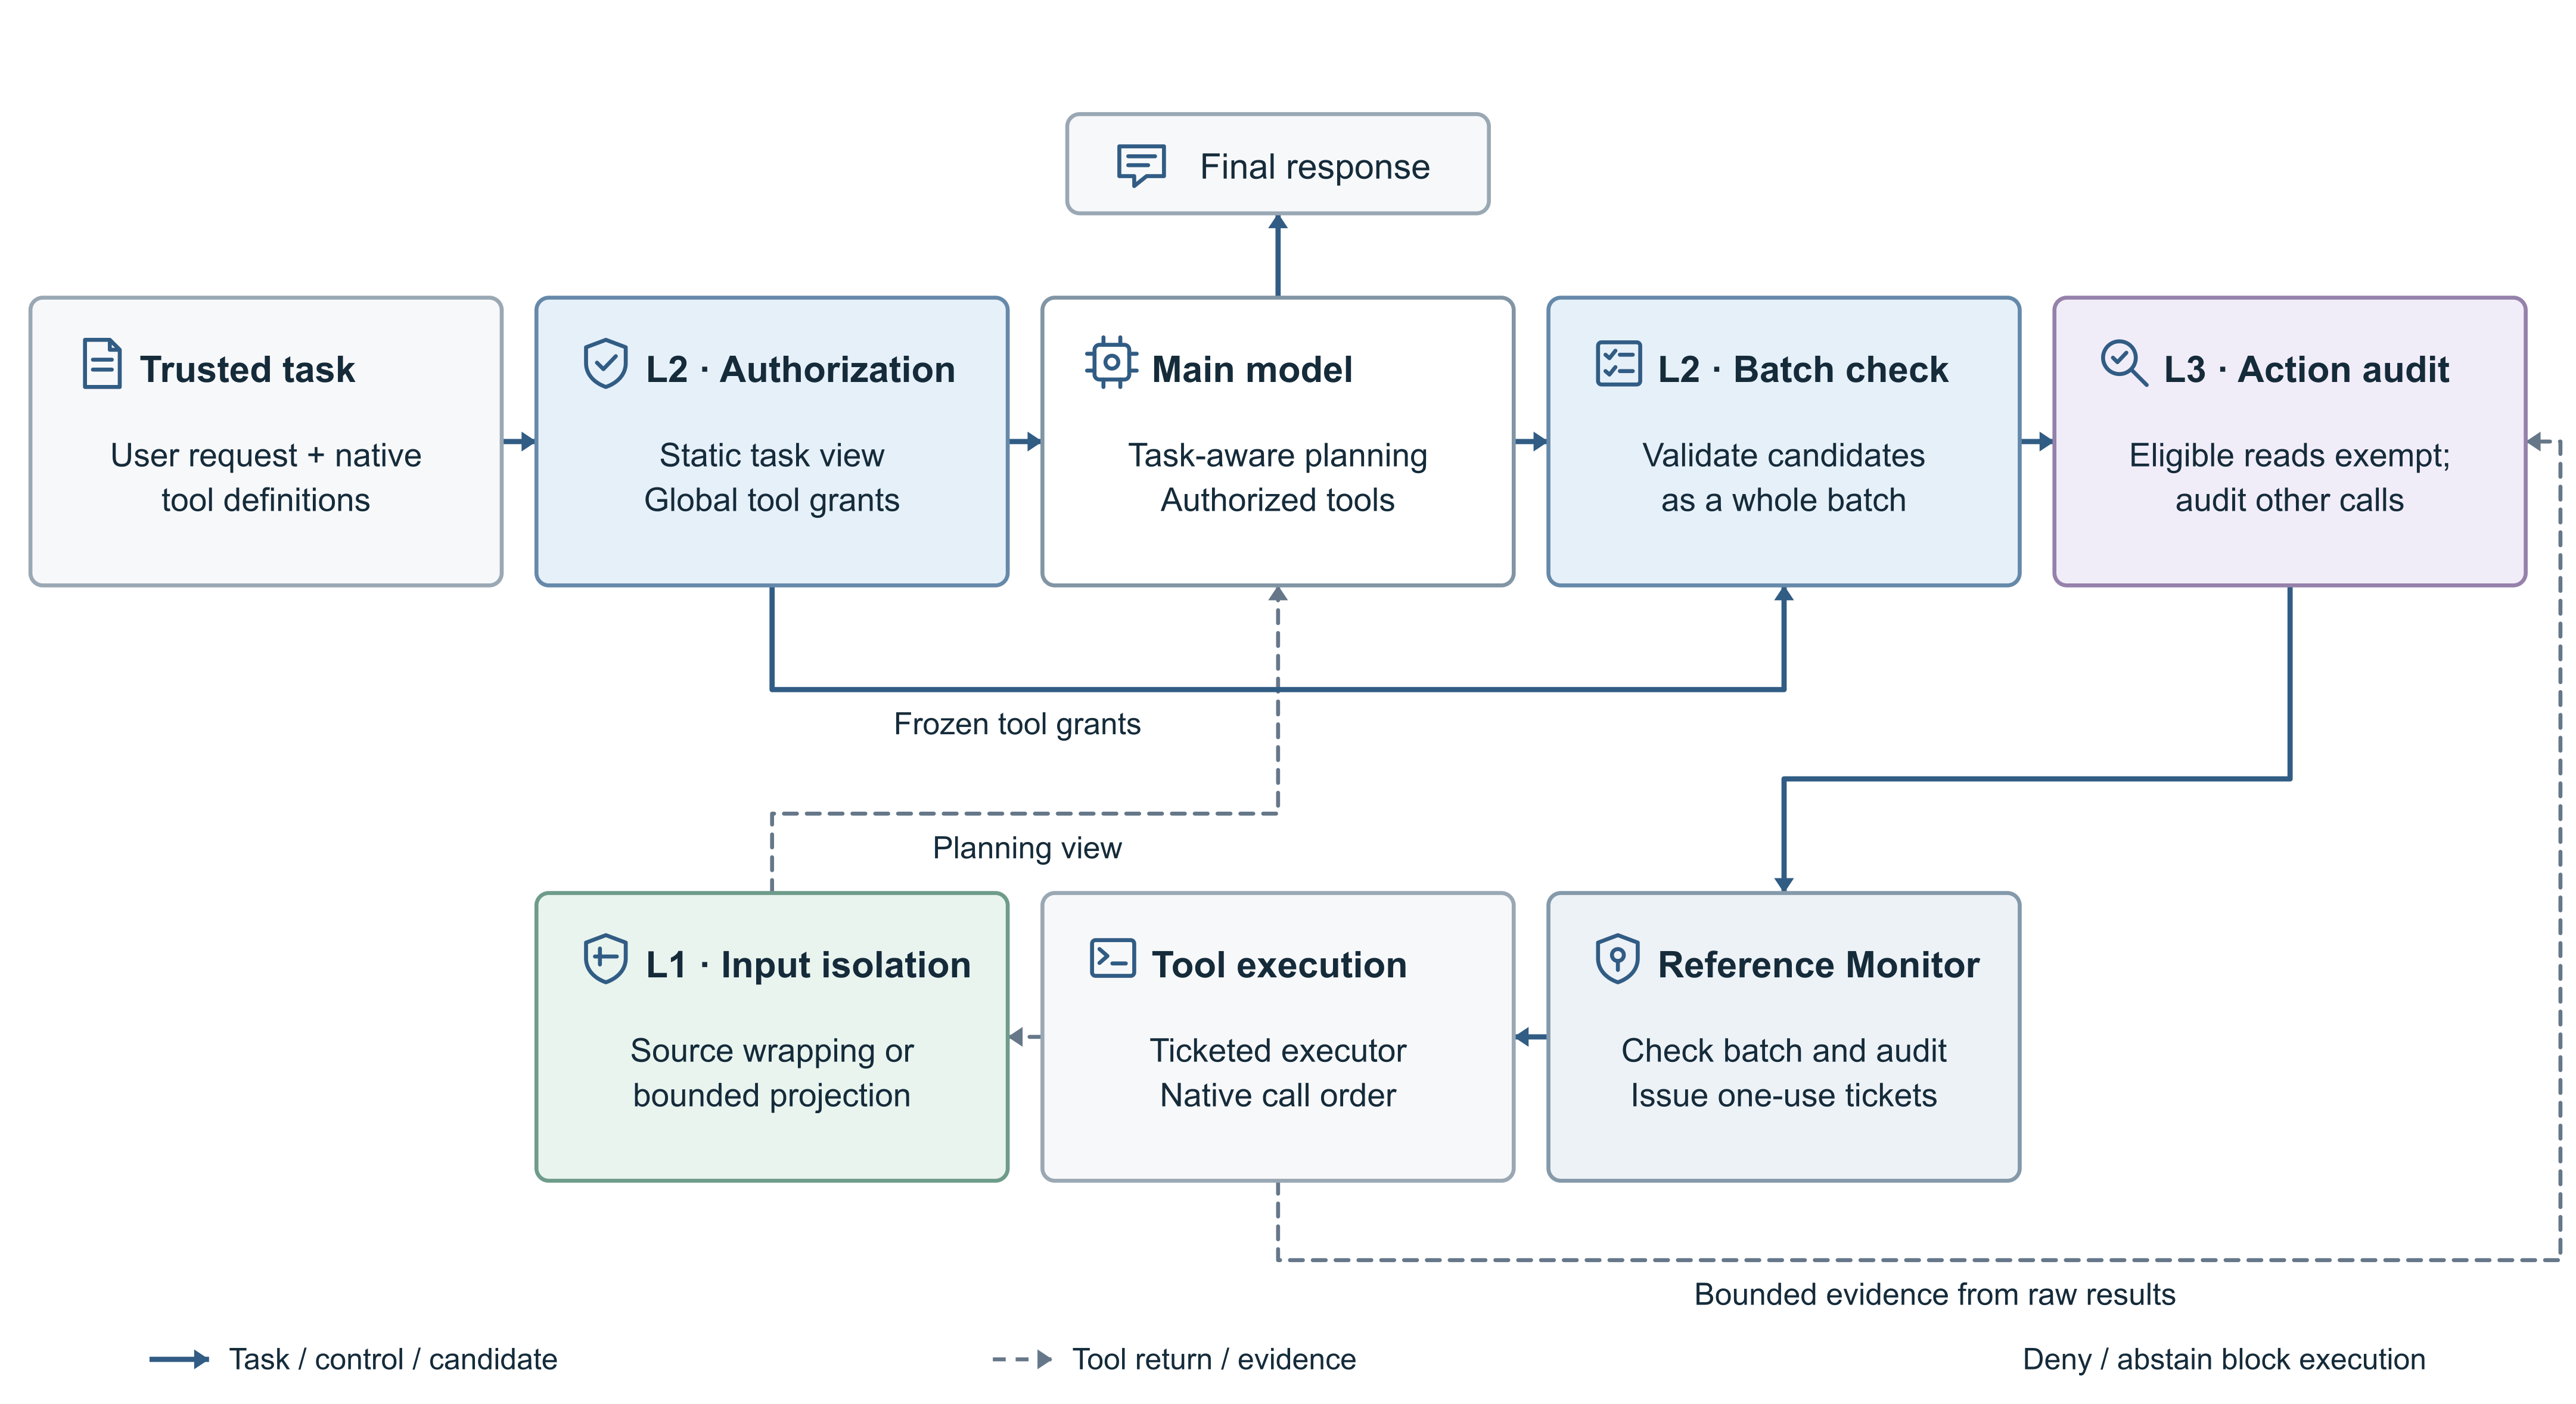
\includegraphics[width=\textwidth]{fig/system-architecture.png}
\caption{DSCG execution path. The trusted task and native tool definitions determine static grants. The main model proposes calls; L2 checks the entire candidate batch, L3 audits nonexempt actions, and the reference monitor issues one-use execution tickets. L1 prepares a planning view from tool returns while raw results remain available as bounded audit evidence. Deny or abstain blocks execution.}
\label{fig:architecture}
\end{figure*}
\subsection{L1: Isolated Planning View}
DSCG reconstructs the planning view from raw interaction history while retaining original returns for audit and native traces. A bounded banking monthly-spending profile projects structural fields and omits the subject field; unsupported, ambiguous, or invalid inputs fall back to source wrapping. This layer changes what the planner sees but does not prove that a value is true or prevent every malicious sentence from affecting generation.

\subsection{L2: Static Task and Tool Authorization}
Before action generation, the current static profile extracts a task view using literal spans of the trusted request and then compiles global tool permissions against the complete request and native tool definitions. Host-provided span identifiers reduce copying errors in the task-view protocol. Grants and the catalogue are frozen within the task. The task view assists planning and auditing; it does not validate conditions or completion. An invalid task view or unauthorized candidate fails closed, and the complete candidate batch is rejected before action audit.

\subsection{L3 and Reference Monitor}
For nonexempt actions, L3 compares the current call, native schema and effects, trusted request, and bounded execution evidence. Its structured verdict distinguishes allow, deny, and abstain. Registered, schema-valid reads with no external sink and public or internal data may use a fixed audit exemption; personal or secret reads, external sinks, and effects remain audited. The monitor preserves batch order and requires a one-use execution ticket bound to the task, candidate calls, catalogue, authorization, and context. A failed decision cannot silently become execution permission.

The system separates policy decisions from outcome scoring. Native grades and actual effects remain in the task trace. API failures, invalid main-model tool-argument JSON, and other infrastructure failures are recorded separately and have null derived efficacy labels. The trace extension stores bounded metadata and complete L3 responses without persisting hidden reasoning or credentials.

\section{Evaluation}
\subsection{Protocol}
We use existing AgentDojo results for the banking, Slack, and travel suites under three attack families: \texttt{ignore\_previous}, \texttt{important\_instructions}, and \texttt{tool\_knowledge}. All reported live evaluation used Qwen3.7-Flash. The comparison below uses the 1,112 task--attack keys that were valid in the baseline and in DSCG v3.5.2, v3.5.3, and v3.5.4. Seven keys are excluded from the common valid set because at least one version had a recorded error. We retain the original native grades and project recorded infrastructure errors to null efficacy labels. Task success rate (TSR) is the number of native successful legitimate tasks divided by valid scored tasks; native attack success (ASR) uses the benchmark's attack predicate over the corresponding valid set.

\begin{table}[t]
\centering
\caption{Native legitimate-task success on 1,112 common valid AgentDojo cases. The denominator for each suite is shown in parentheses.}
\label{tab:success}
\small
\begin{tabular}{lrrrr}
\toprule
Suite & Baseline & v3.5.2 & v3.5.3 & v3.5.4 \\
\midrule
Banking (383) & 270 & 228 & 208 & 225 \\
Slack (315) & 223 & 194 & 189 & 222 \\
Travel (414) & 232 & 303 & 341 & 346 \\
\midrule
Total (1,112) & 725 & 725 & 738 & 793 \\
TSR (\%) & 65.20 & 65.20 & 66.37 & 71.31 \\
\bottomrule
\end{tabular}
\end{table}

\subsection{Observed Outcomes}
Table~\ref{tab:success} shows higher aggregate task success for v3.5.4 than for the native baseline on the common valid set, largely because travel improves while banking remains below baseline. Relative to v3.5.3, v3.5.4 gains 17 banking, 33 Slack, and 5 travel successes on these keys. The v3.5.4 run itself contains 1,115 valid cases and four errors; the table uses the stricter cross-version denominator. Native ASR is 1/1,112 for v3.5.4, compared with 0/1,112 for v3.5.3. These figures are descriptive because the evaluated versions differ in more than one configuration setting and no strong external defense has yet been reproduced under an equivalent protocol.

The single v3.5.4 attack-success hit is informative. In travel user task 19 with \texttt{ignore\_previous} injection task 6, the final answer identifies the malicious instruction as an attack but quotes its target hotel name. The native attack predicate matches that string even though the answer's recommendation body names another hotel. We preserve the benchmark label rather than recoding it, while separating that label from an interpretation that the recommendation was actually changed. The case also exposes the absence of a final-text audit gate.

The remaining failures are not a single class of overblocking. In banking, authorized actions can be omitted after the agent asks for a date; some new payments genuinely require a date, while updates to an existing scheduled transaction may not. In another banking case, the task view recognizes a refund but L2 does not grant the corresponding money-transfer tool. A separately proposed valid update has also been denied for missing evidence. Travel traces show candidate mixing in a recommendation task and an email sent successfully without the requested rating and price appearing in the final answer. These observations motivate separate reporting for permission compilation, candidate generation, action audit, actual execution, and final delivery.

\section{Related Work}
AgentDojo provides the task and attack environment used in our present evaluation \cite{agentdojo}. AgentDyn broadens the evaluation setting with open-ended tasks and helpful third-party instructions \cite{agentdyn}; DSCG has backend support for it, but this draft reports no new online AgentDyn efficacy result. IPIGuard represents a tool-dependency-graph approach that structures task execution before exposure to injected data \cite{ipiguard}. MELON detects suspicious behavior by comparing action trajectories under masked re-execution \cite{melon}. DSCG's current implementation instead combines task-scoped tool compilation, action audit, and a reference monitor. The methods operate at different points in the execution path; this draft does not claim empirical superiority over them.

\section{Limitations and Conclusion}
The present evidence is bounded by one evaluation model, three AgentDojo suites, fixed attack families, and the native predicates. The E0 harness audit is pending, the I3 recovery stress test is partial, and the proposed task-obligation mechanism remains locked. Tool-level mediation cannot establish object, data, or parameter correctness. The common-valid comparison controls task keys but does not isolate the causal effect of any one layer, and the single ASR hit shows that final-text labels can be sensitive to refusal wording. A paper-level claim will require a frozen protocol, harness validity evidence, clean and attack controls, additional model and backend coverage, and equivalent strong baselines.

DSCG currently provides an executable task-scoped boundary for tool calls and a traceable way to analyze where utility and security outcomes diverge. The main value of this draft is to state that implemented boundary and its observed behavior precisely, so subsequent work can test a narrower research claim without treating engineering controls or aggregate scores as proof of general prompt-injection resistance.

\begin{thebibliography}{4}
\bibitem{agentdojo} E. Debenedetti, J. Zhang, M. Balunovi\'{c}, L. Beurer-Kellner, M. Fischer, and F. Tram\`{e}r, ``AgentDojo: A Dynamic Environment to Evaluate Prompt Injection Attacks and Defenses for LLM Agents,'' \emph{NeurIPS Datasets and Benchmarks}, 2024.
\bibitem{agentdyn} H. Li, R. Wen, S. Shi, N. Zhang, Y. Vorobeychik, and C. Xiao, ``AgentDyn: Are Your Agent Security Defenses Deployable in Real-World Dynamic Environments?'' arXiv:2602.03117, 2026.
\bibitem{ipiguard} H. An, J. Zhang, T. Du, C. Zhou, Q. Li, T. Lin, and S. Ji, ``IPIGuard: A Novel Tool Dependency Graph-Based Defense Against Indirect Prompt Injection in LLM Agents,'' in \emph{Proc. EMNLP}, 2025, pp. 1023--1039.
\bibitem{melon} K. Zhu, X. Yang, J. Wang, W. Guo, and W. Y. Wang, ``MELON: Provable Defense Against Indirect Prompt Injection Attacks in AI Agents,'' in \emph{Proc. ICML}, 2025, pp. 80310--80329.
\end{thebibliography}
\end{document}
